\documentclass[a4paper,10pt]{report}
\usepackage[utf8x]{inputenc}
\usepackage{amsmath}
\usepackage{graphicx}
%\usepackage{abssymb}
%opening
\title{Draft 1}
\author{Anupam Prasad Vedurmudi}

\begin{document}

\maketitle

\begin{abstract}
 
\end{abstract}

\section{Scattering Theory}

\subsection{Formal Scattering Theory}
The spectrum of any 

We define the Hamiltonian operator as,
\begin{equation}
 H = H_0+V\\
\end{equation}
\noindent Where, $H_0$ is the free Hamiltonian given by, 

\begin{equation}
 H_0=-\frac{\Delta}{2}
\end{equation}
\noindent $V$ is the potential.

\noindent The Green's function is formally defined as,
\begin{eqnarray}\label{GFdefinition}
 G\left(E+i\epsilon\right) &=\left(E+i\epsilon-H\right)^{-1}\\
 G_0\left(E+i\epsilon\right) &=\left(E+i\epsilon-H_0\right)^{-1}
\end{eqnarray}

\noindent The Lippmann-Schwinger equation for the Green's function is given by,
\begin{equation}\label{LS1}
 G=G_0+G_0VG
\end{equation}

\noindent Subsequently, the Born series for $G$ is obtained by recursively substituting
the $(n-1)^{th}$ order approximation for $G$ in the R.H.S of \eqref{LS1} to get the $n^{th}$
order term. The $0^{th}$ order approximation is the free Green's function $G_0$, the $1^{st}$
order approximation (the Born approximation) is given by,

\begin{equation}\label{BornApproximation}
 G=G_0+G_0VG_0
\end{equation}

The Born series can thus be written as,

\begin{equation}\label{BornSeriesExpanded}
 G=G_0+G_0VG_0+G_0VG_0VG_0+\ldots
\end{equation}

\noindent Or more compactly,
\begin{equation}\label{BornSeriesCompact}
 G=\displaystyle\sum_{n=0}^{\infty}G_0\left(VG_0\right)^n
\end{equation}

\section{Finite Element Method}
The Finite Element Method (FEM) is a numerical technique used to solve differential equations.
The method exploits the locality of the differential operator. The solution space is divided into
subspaces. These subspaces take the form of a mesh, i.e., a collection of simplices - triangles
in 2D, tetrahedra in 3D, etc. The function is then approximated using smooth basis functions with support in these subspaces.
These basis functions with finite support are referred to as finite elements.

Let $\psi$ be a solution to a differential equation. We denote the basis functions by $\phi_n$,
\begin{equation}\label{femfirst}
 \psi(\mathbf{x})\simeq\widetilde{\psi}(\mathbf{x})=\displaystyle\sum_n^N c_n\phi_n(\mathbf{x})
\end{equation}

A feature of FEM is that the basis functions have a finite overlap i.e., they are not orthogonal.
The overlap matrix in general has a block-diagonal form. The overlap matrix is denoted by,
\begin{equation}\label{overlap}
 S_{nm}=\int d^3x\phi_n(\mathbf{x})\phi_m(\mathbf{x})
\end{equation}

We also define the matrix,
\begin{equation}\label{diff_overlap}
 B_{nm}=\int d^3x\nabla\phi_n(\mathbf{x}).\nabla\phi_m(\mathbf{x})
\end{equation}

\subsection{Boundary Conditions}
In order to solve the differential equations we must also specify appropriate boundary
conditions. Let $\Omega$ be the solution space. We denote its boundary by $\partial\Omega$.

\subsubsection{Dirichlet Boundary Condition}
The Dirichlet boundary condition requires that the function has a known value on the boundary.
\begin{equation}\label{dirichlet1}
 \psi(\mathbf{x})=f(\mathbf{x}), \mbox{ }\forall\mathbf{x}\in \partial\Omega
\end{equation}
Where, $f$ is a known function on $\Omega$.

\subsubsection{Neumann Boundary Condition}
The Neumann boundary condition requires that the gradient of the function
normal to the boundary is fixed to a known function. That is,
\begin{equation}\label{neumann1}
 \frac{\partial\psi(\mathbf{x})}{\partial\mathbf{n}}\equiv\nabla\psi(\mathbf{x}).\mathbf{n} = f(\mathbf{x}), \mbox{ }\forall\mathbf{x}\in \partial\Omega
\end{equation}

\subsubsection{Mixed Boundary Condition}
It is also possible to have a boundary such that the function has a Dirichlet boundary
condition on one part (denoted by $\partial\Omega_D$) and a Neumann boundary condition
on the other ($\partial\Omega_N$).

\subsection{Python Implementation}
\section{FEM in Quantum Mechanics}
The Schrödinger equation for a wave function $\psi$ is given by,

\begin{equation}\label{schroedinger1}
 -\frac{\Delta}{2}\psi+V(\mathbf{x})\psi=E\psi
\end{equation}

\noindent Using the FEM approximation defined in \eqref{femfirst},
\begin{equation}\label{schroedinger}
 -\frac{\Delta}{2}\displaystyle\sum_n^N c_n\phi_n(\mathbf{x})+\displaystyle\sum_n^N c_n V(\mathbf{x})\phi_n(\mathbf{x})=E\displaystyle\sum_n^N c_n\phi_n(\mathbf{x})
\end{equation}
\noindent We get the weak formulation of the problem by multiplying both sides by $\phi_m(\mathbf{x})$ and integrating over. After integrating by parts, the kinetic term gives us
the following matrix element,
\begin{equation}\label{kineticterm}
 \int d^3x\phi_m(\mathbf{x})\Delta\phi_n(\mathbf{x}) = -\int d^3x\nabla\phi_m(\mathbf{x}).\nabla\phi_n(\mathbf{x}) = -B_{mn}
\end{equation}

\noindent The potential term is calculated from the known functions $\phi_n$ and is defined as,
\begin{equation}\label{potentialterm}
 \int d^3xV(\mathbf{x})\phi_m(\mathbf{x})\phi_n(\mathbf{x}) = V_{mn}
\end{equation}

\noindent Finally, the R.H.S is given by,
\begin{equation}
 E\int d^3x\phi_m(\mathbf{x})\phi_n(\mathbf{x})=ES_{mn}
\end{equation}

\noindent We define the coefficient vector $\mathbf{\underline{c}}=[c_1,c_2,\ldots,c_N]^T$. The Schrödinger equation reduces to 
the following eigenvalue problem,
\begin{equation}\label{schroedingerfem}
  H\mathbf{\underline{c}}=ES\mathbf{\underline{c}}
\end{equation}
\noindent Where, $H=\left(\frac{B}{2}+V\right)$

The inner product of two wavefunctions $\phi$ and $\chi$ is given by,
\begin{eqnarray}\label{innerproduct}
 \int d^3x \chi^*(\mathbf{x})\psi(\mathbf{x}) &=& \displaystyle\sum_{m,n}^{N}c_md_n\int d^3x \phi_m(\mathbf{x})\phi_n(\mathbf{x})\\
 &=& \mathbf{c}^{\dagger}S\mathbf{d}
\end{eqnarray}
\noindent Where, $\mathbf{c}^{\dagger}=(\mathbf{c}^*)^T$.

\subsection{Momentum Eigenstates}
We now want to find an FEM representation for free eigenstate of momentum $\mathbf{k}$ (energy,
$E_k=|\mathbf{k}|^2/2$). 
It is most convenient to do so by defining a ``cosine eigenvector'',
\begin{equation}\label{cosevec}
 |\mathbf{k}\rangle = exp(-i\mathbf{k}.\mathbf{x}) + exp(i\mathbf{k}.\mathbf{x})
\end{equation}
These can be obtained by ``solving'' the free Schrödinger equation on a grid with open
boundaries, i.e., by solving the eigenvalue problem,

\begin{equation}\label{freeschroedinger}
 H_0\psi=\lambda S\psi
\end{equation}
for $\psi$.

$|\mathbf{k}\rangle$ has the following properties,
\begin{eqnarray}
 \langle\mathbf{k}|S|\mathbf{k}\rangle &=&\int_{\Omega} d^3x\\
 \langle\mathbf{k}^{\prime}|S|\mathbf{k}\rangle &\simeq& 0
\end{eqnarray}
Here, $\int_{\Omega} d^3x$ is the volume of the solution space.

\subsection{Born Series - FEM Formulation}
We calculate the FEM representation of the Greens Function using \eqref{schroedingerfem}. We require that,
\begin{equation}\label{greenfemreq}
 G_{fem}(z)\psi=(z-E_0)^{-1}S\psi
\end{equation}
\noindent Where, $\psi$ is an eigenstate of $H$ of energy $E_0$. Thus, we define the Green's function as,
\begin{equation}\label{greenfemdef}
 G_{fem}(z)=\left(z\mathbf{I}-HS^{-1}\right)^{-1}S
\end{equation}
\noindent Where, $\mathbf{I}$ is the identity matrix. The free Greens function is defined similarly by setting
$H=B/2$. We will ultimately be testing the convergence of, $\langle\mathbf{k}|G_{fem}(z)|\mathbf{k}\rangle$.
For later convenience, the potential matrix is also suitably modified as,
\begin{equation}\label{potmat}
 V_{fem}=S^{-1}VS^{-1}
\end{equation}


\subsection{Modification of the Hamiltonian}
In this section we use the techniques outlined in \cite{KukPom76}. It this paper, the Born
series is rearranged by using orthogonally projecting pseudopotentials (OPP). It is then
proved that the rearranged Born series converges for all negative and small positive energies
even if the system contains bound states.

Let the bound states (indexed by $a$) of the Hamiltonian $H$ be denoted by $|\psi_a\rangle$.
The potential is modified by the operator $\Gamma$ given by,
\begin{equation}\label{potmod}
  \Gamma=\lambda\displaystyle\sum_a |\psi_a\rangle\langle\psi_a|
\end{equation}
\noindent The rate of convergence of the Born series is controlled by the parameter $\lambda$.

The modified Hamiltonian and the modified free Hamiltonian are denoted by,

\begin{eqnarray}
 \widetilde{H}&=&H+\Gamma\\
 \widetilde{H}_0&=&H_0+\Gamma
\end{eqnarray}

The modified Greens functions $\widetilde{G}$ and $\widetilde{G}_0$ are defined similarly as
in \eqref{GFdefinition}. The modified Born Series for $\widetilde{G}$ is given by,

\begin{equation}\label{BornSeriesModCompact}
 \widetilde{G}=\displaystyle\sum_{n=0}^{\infty}\widetilde{G}_0\left(V\widetilde{G}_0\right)^n
\end{equation}

\noindent Physically, this means that the modified Hamiltonian has the same continuous spectrum but the discrete
spectrum has been shifted by $\lambda$.

\section{Toy Problem - Scattering in 1D}
We now use the above methods in an example with scattering off a potential in 1D. Due to the simplicity of the problem,
it is possible to explicitly calculate the exact Green's function by inverting the appropriate matrix according the formal
definition given in \eqref{GFdefinition}. We will examine the problem in three cases: 
\begin{itemize}
 \item In the first case, we have convergence with both the modified and unmodified Hamiltonian but at a faster rate with the modification.
 \item In the second case, the unmodified case converges for certain energies and diverges for others.With the modification, we always have
       faster convergence.
 \item In the third case, the modified hamiltonian gives a convergent Born series whereas the unmodified one diverges. 
\end{itemize}

Our box is defined as an FEM axis from $x=0$ to $x=10$ with $n=400$ discretization points, 
of order $40$ and with open boundaries. This means that the axis is divided into 400 
parts and each part has functions (elements) upto order $40$. Order $1$ being a straight
line. As an example, we show an axis, $0\leq x\leq 4$ with $n=4$ discretization points, open
boundaries and order $1$.

\begin{figure}[hm]
\centering
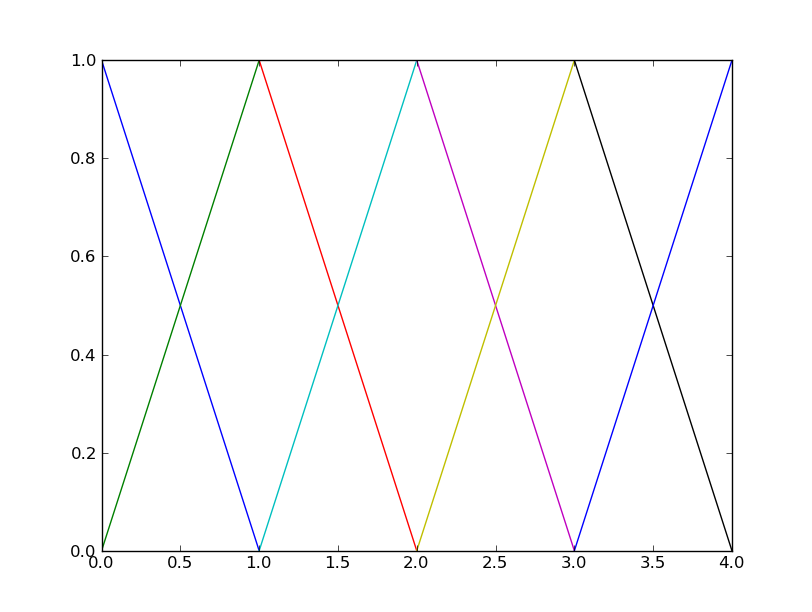
\includegraphics[width=225pt, height=150pt]{femexample1.png}
\caption[\textwidth]{FEM axis. n=4, order=1}
\end{figure}
The different elements are distinguished by colour.

The ``cosine eigenvectors'' are computed using \eqref{cosevec} and \eqref{freeschroedinger}.
The energies of the free wavefunctions are $E_n = n^2\pi^2/200$ for $n=0,\ldots,19$. The factor
of $200$ is a result of the discretization. The Green's function, $G(z)$ is calculated for $z=E_n+i\epsilon$,
where, $\epsilon$ is a small positive number defined based on the problem. The purpose of epsilon is to avoid 
the singularity on the positive real axis.

\subsection{First Case}
In the first case, we define the potential as a finite well of strength $0.1$ with support in $4 \leq x \leq 6$,
\begin{equation}\label{potentialdef1}
V = \begin{cases}
-0.1 &\mbox{} 4\leq x\leq 6\\
0 &\mbox{ otherwise}
\end{cases} 
\end{equation}

\begin{figure}[ht]
\centering
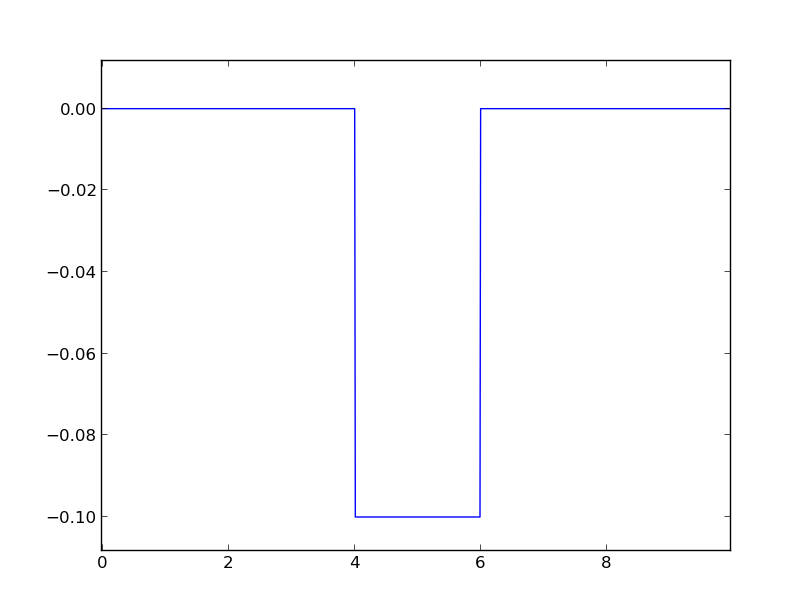
\includegraphics[width=225pt, height=150pt]{potential1d1.png}
\caption[\textwidth]{Test Potential 1}
% 
% \centering
% 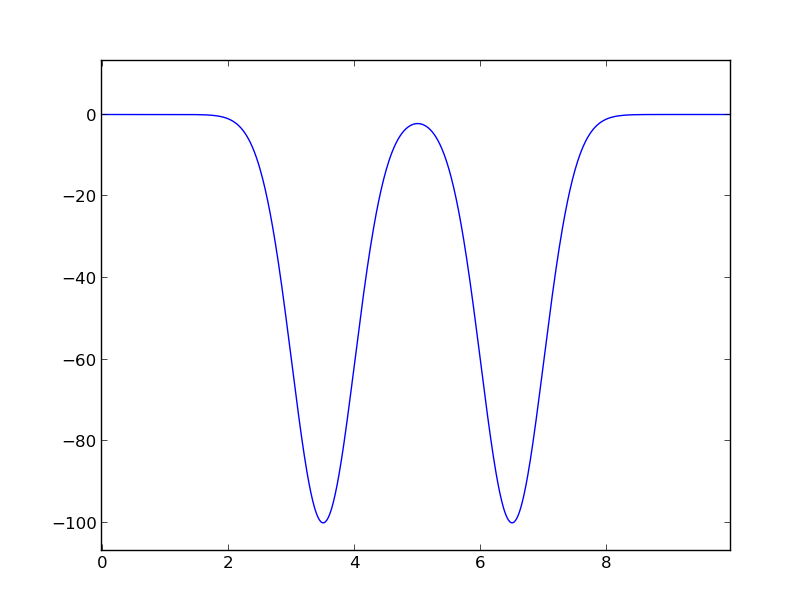
\includegraphics[width=225pt, height=150pt]{potential1d2.png}
% \caption[\textwidth]{Test Potential 2}
\end{figure}

The Born Series is calculated for $15$ iterations. The Hamiltonian is modified using the operator defined in \eqref{potmod} with
$\lambda=1$.  We also set $\epsilon=0.1$. 

We now plot the elements of the Born Series against the number of iterations. In order
to compare the modified and unmodified cases, we plot them side by side with the modified case on the left and the unmodified one
on the right. We follow this convention in the other two cases as well.

\begin{center}
\begin{figure}[lht]
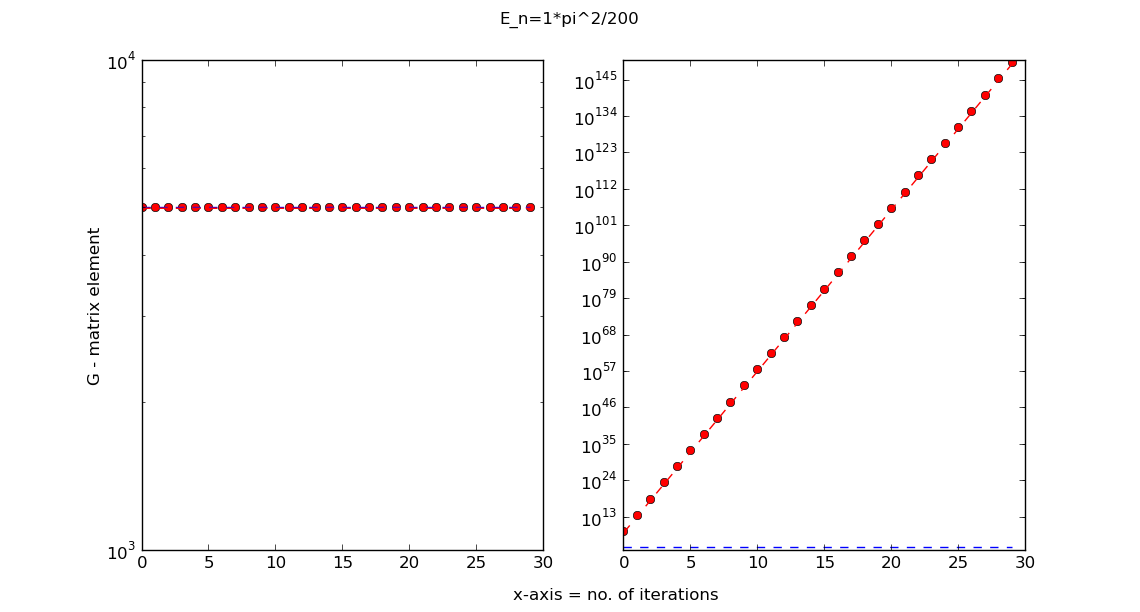
\includegraphics[width=360pt, height=200pt]{series1a.png}
%\caption[\textwidth]{First Case}
\end{figure}
\end{center}

\begin{center}
\begin{figure}[lht]
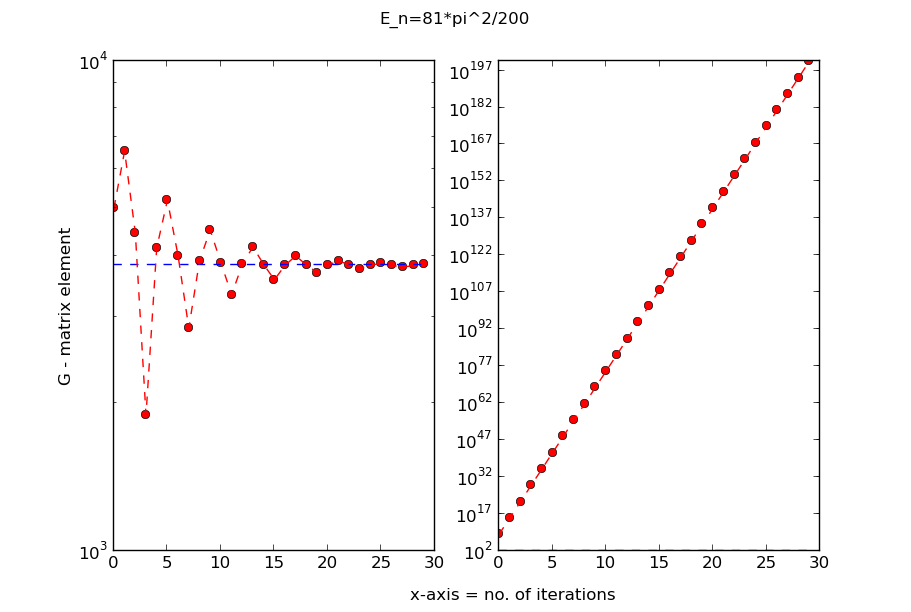
\includegraphics[width=360pt, height=200pt]{series1b.png}
%\caption[\textwidth]{First Case}
\end{figure}
\end{center}

\begin{center}
\begin{figure}[lht]
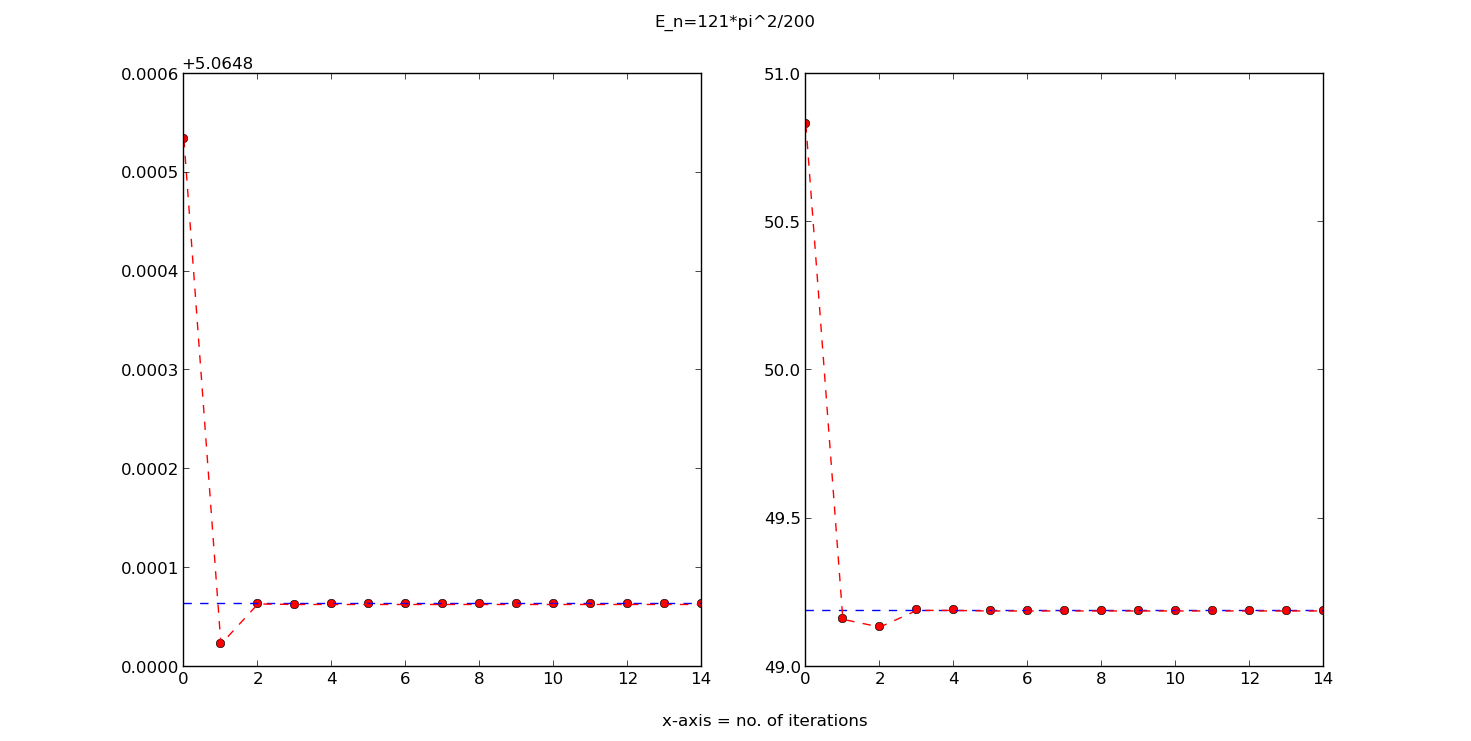
\includegraphics[width=360pt, height=200pt]{series1c.png}
%\caption[\textwidth]{First Case}
\end{figure}
\end{center}

We see that the Born Series converges to the exact value in both cases. It is also to be noted that the 
.

\subsection{Second Case}
In the second case, we define the potential as, 
\begin{equation}\label{potentialdef2}
V = \begin{cases}
-0.5 &\mbox{} 4\leq x\leq 6\\
0 &\mbox{ otherwise}
\end{cases} 
\end{equation}

\begin{figure}[hb]
\centering
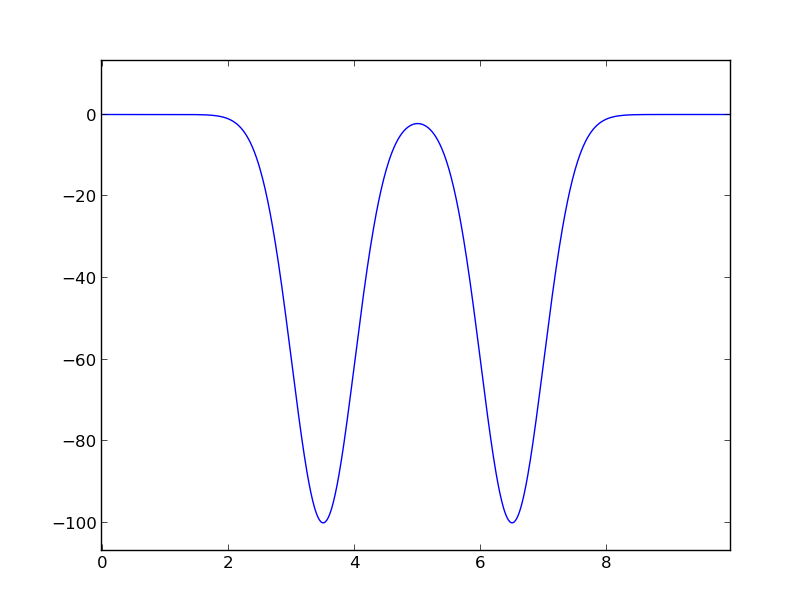
\includegraphics[width=225pt, height=150pt]{potential1d2.png}
\caption[\textwidth]{Test Potential 2}
\end{figure}

The born series is calculated for $15$ iterations. We choose $\lambda=700$ and $\epsilon=10^{-8}$.

\begin{center}
\begin{figure}[lht]
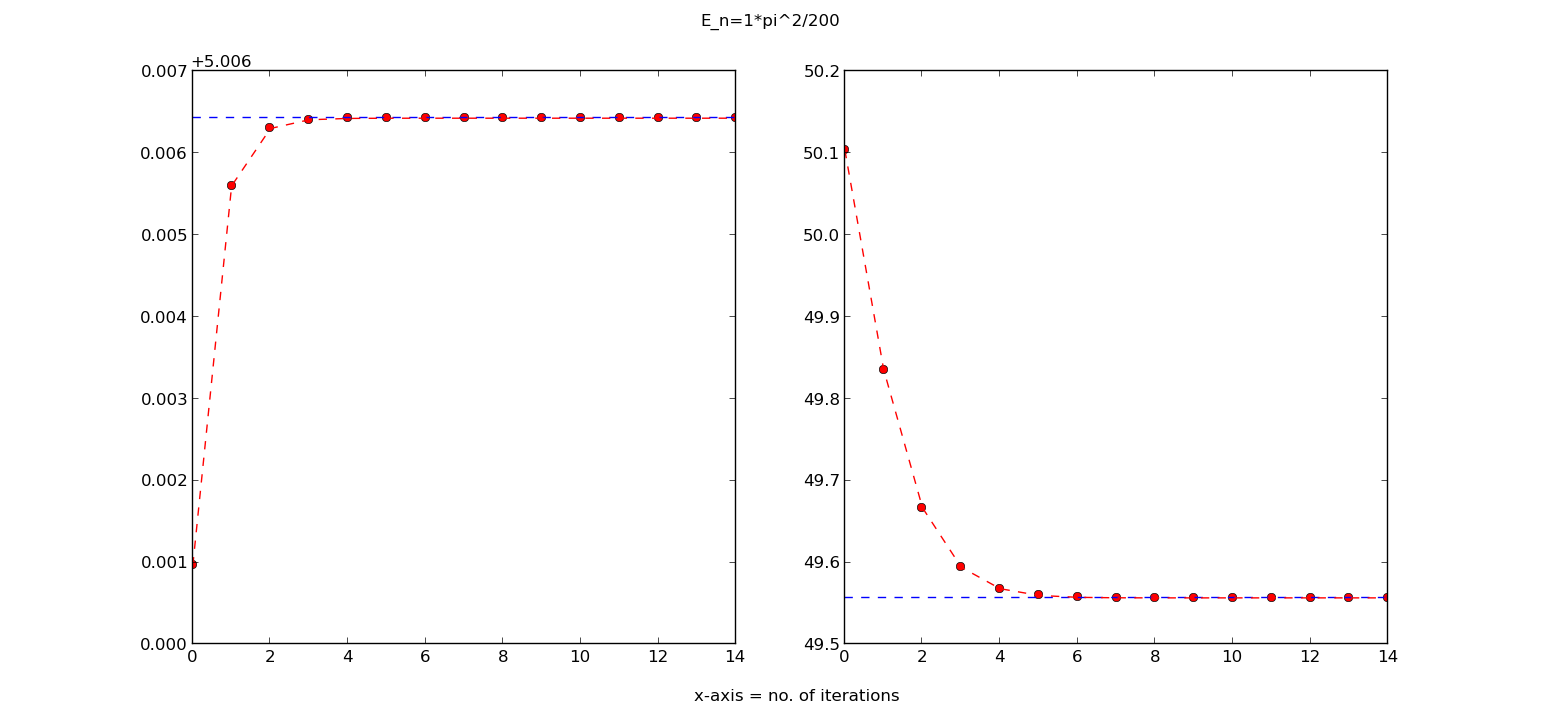
\includegraphics[width=360pt, height=200pt]{series2a.png}
%\caption[\textwidth]{First Case}
\end{figure}
\end{center}

\begin{center}
\begin{figure}[lht]
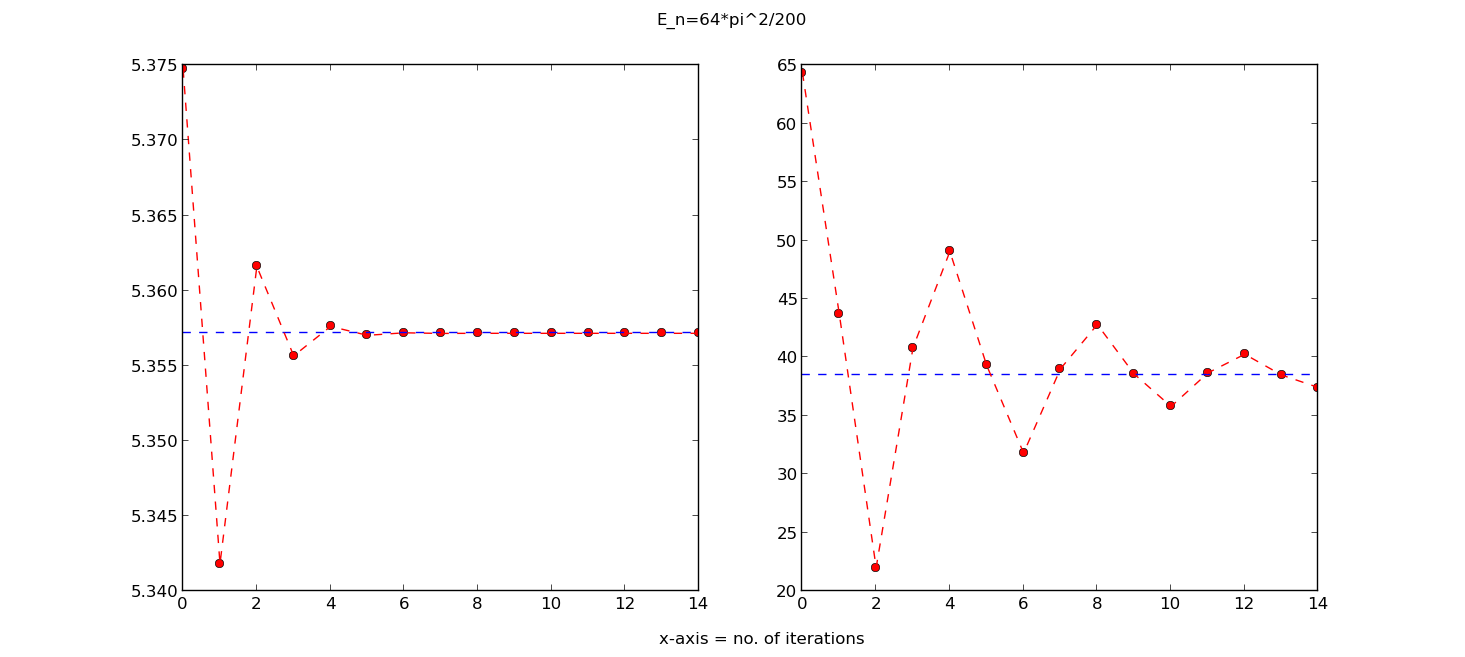
\includegraphics[width=360pt, height=200pt]{series2b.png}
%\caption[\textwidth]{First Case}
\end{figure}
\end{center}

\begin{center}
\begin{figure}[lht]
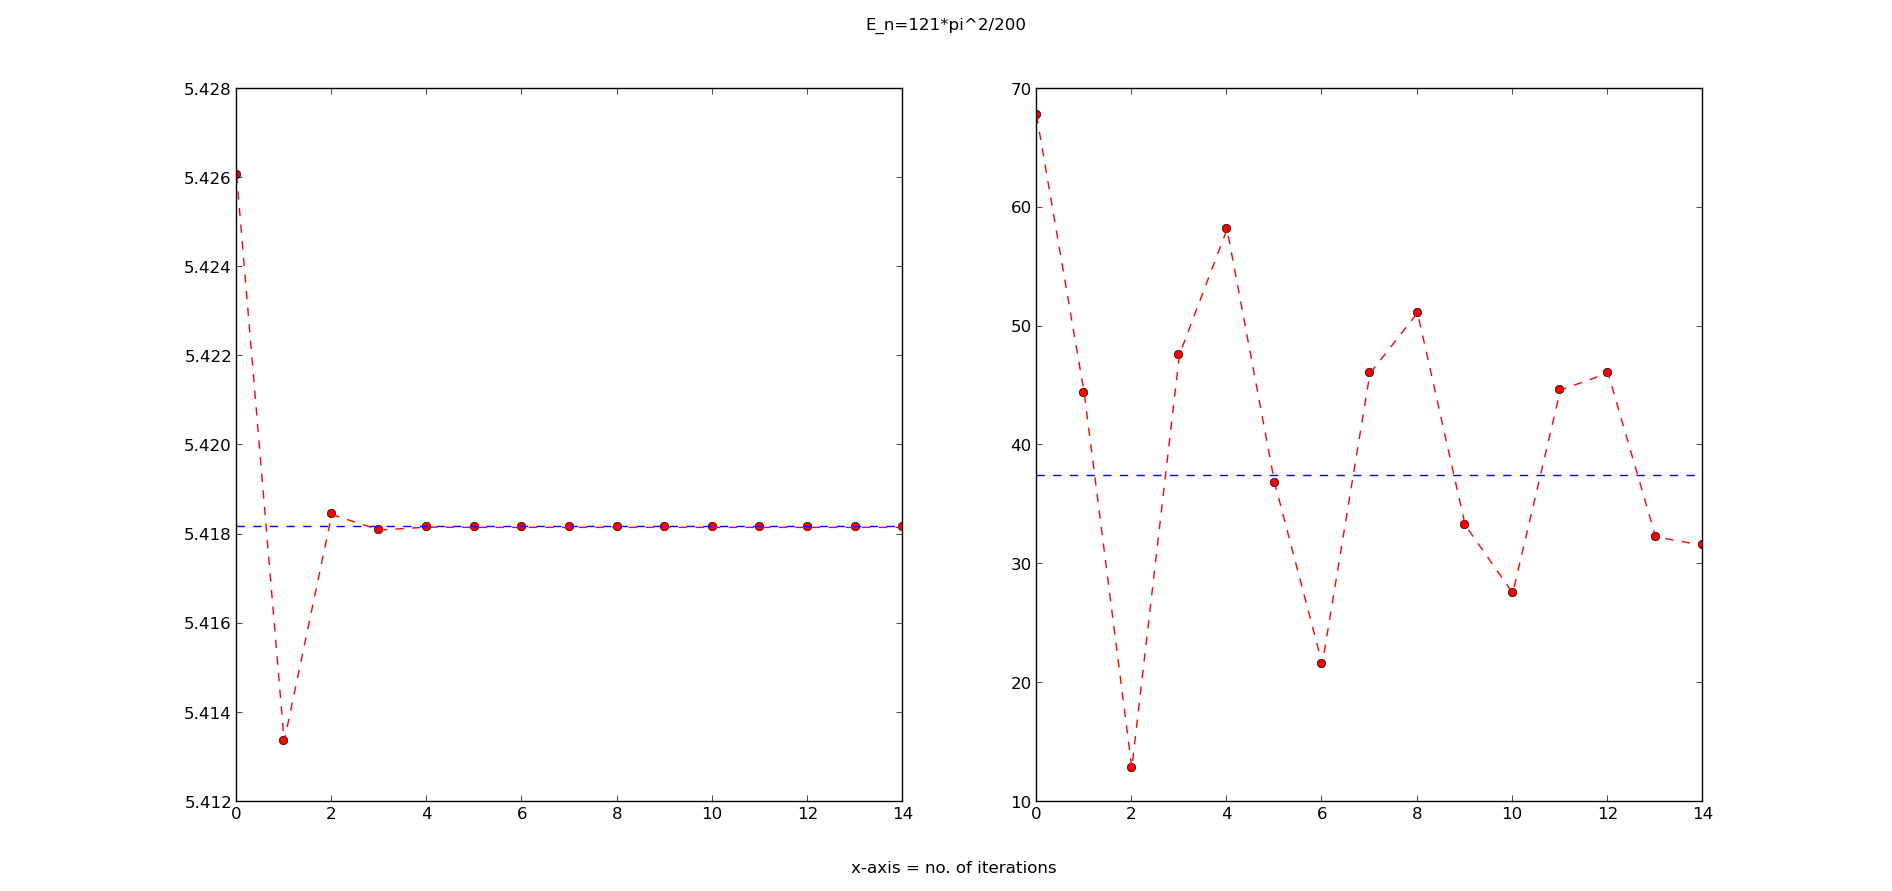
\includegraphics[width=360pt, height=200pt]{series2c.png}
%\caption[\textwidth]{First Case}
\end{figure}
\end{center}

We see that for the original Hamiltonian, the Born series converges in some cases but doesn't in others. However,
with the modification, we always have convergence at a faster rate.
\subsection{Third Case}
\begin{equation}\label{potentialdef2}
V = -200\mathtt{exp}(-(x-3.5)^2/0.5)-200\mathtt{exp}(-(x-6.5)^2/0.5)
\end{equation}

\begin{center}
\begin{figure}[lht]
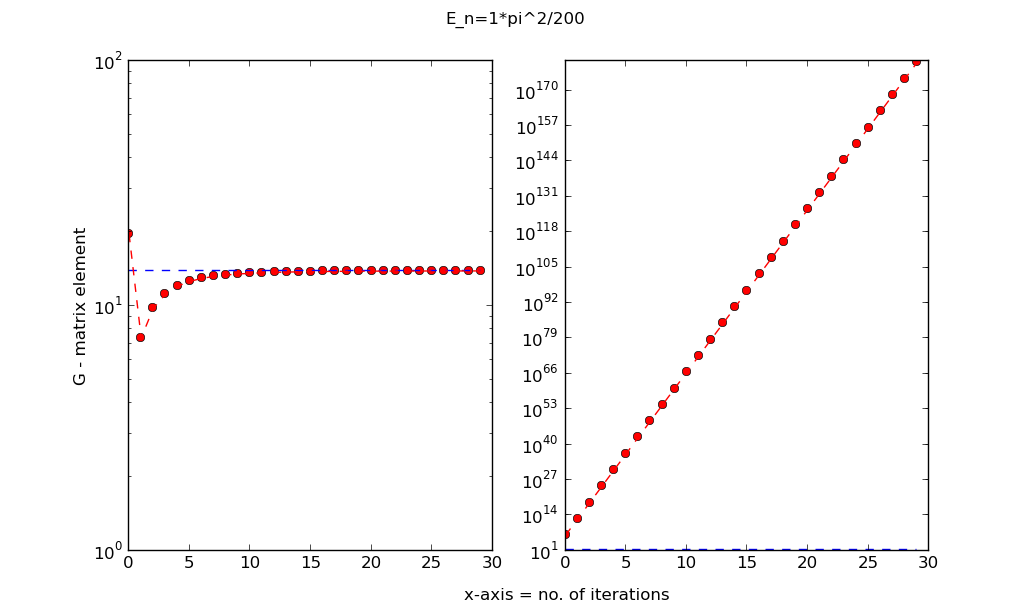
\includegraphics[width=360pt, height=200pt]{series3a.png}
%\caption[\textwidth]{First Case}
\end{figure}
\end{center}

\begin{center}
\begin{figure}[lht]
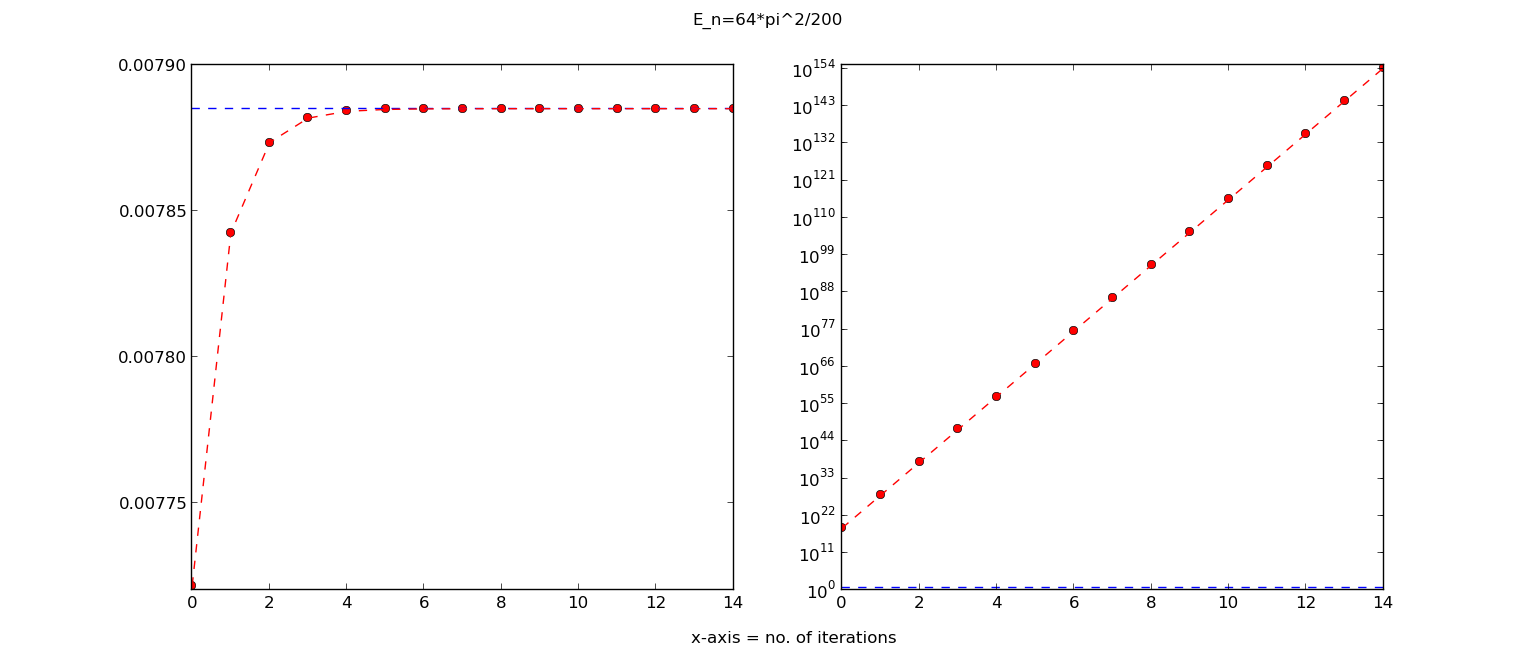
\includegraphics[width=360pt, height=200pt]{series3b.png}
%\caption[\textwidth]{First Case}
\end{figure}
\end{center}

\begin{center}
\begin{figure}[lht]
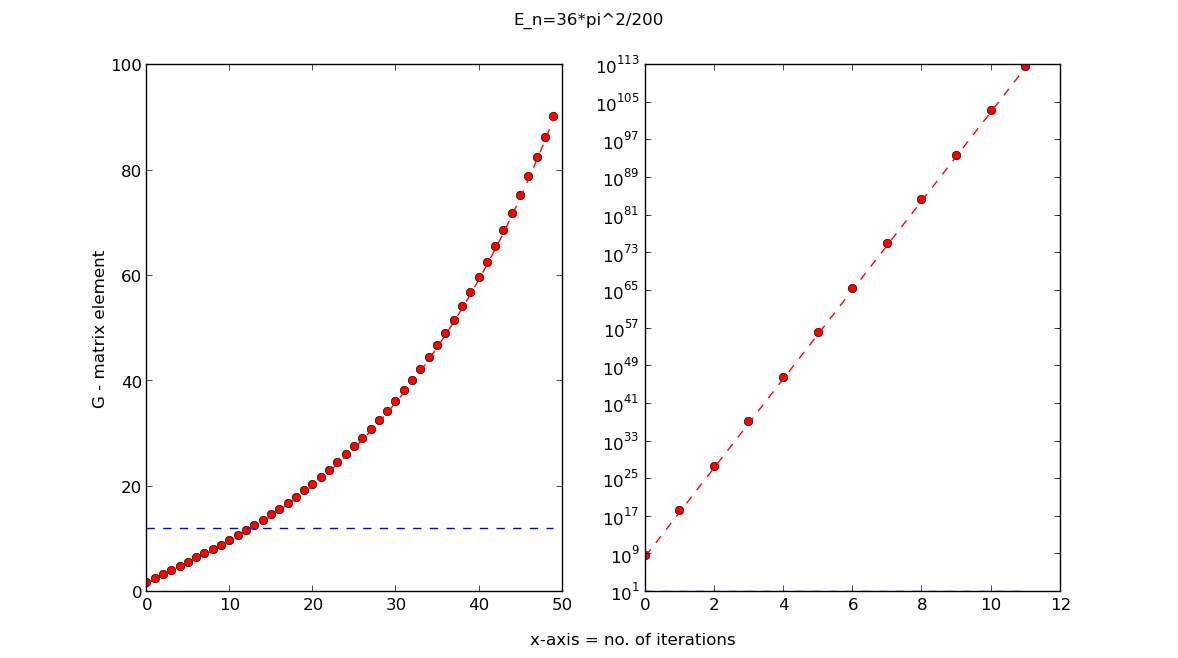
\includegraphics[width=360pt, height=200pt]{series3c.png}
%\caption[\textwidth]{First Case}
\end{figure}
\end{center}

We see that the Born Series in the modified case converges to the exact value but diverges in the original case.
\bibliographystyle{plain}
\bibliography{draft1.bib}
\end{document}
